\documentclass[11pt,a4paper]{article}
\usepackage[utf8]{inputenc}
\usepackage[T1]{fontenc}
\usepackage{lmodern}
\usepackage[french]{babel}
\usepackage[margin=2.2cm]{geometry}
\usepackage{amsmath}
\usepackage{icomma}
\usepackage{graphicx}
\usepackage{booktabs}
\usepackage{caption}
\usepackage{subcaption}
\usepackage[hidelinks]{hyperref}

\captionsetup{font=small}
\setlength{\parskip}{0.4em}

\begin{document}
\begin{center}
{\LARGE Calibration de la caméra principale d'un iPhone 15 Pro}
\end{center}
\vspace{1em}

\section{Objectif et modèle}

Le but de ce TP est de mesurer les paramètres internes de la caméra de mon téléphone, en traitant le capteur comme l'objet d'une expérience. Je suis les tutoriels OpenCV \og Camera Calibration\fg{} et \og Pose Estimation\fg{} en Python, avec OpenCV~5.0.

J'utilise le modèle sténopé vu en cours. Un point $(X,Y,Z)$ du repère de la mire se projette en un pixel $(u,v)$ par
\[
s\begin{pmatrix}u\\v\\1\end{pmatrix}
= K\,[R\,|\,t]\begin{pmatrix}X\\Y\\Z\\1\end{pmatrix},
\qquad
K=\begin{pmatrix}f_x & 0 & c_x\\ 0 & f_y & c_y\\ 0&0&1\end{pmatrix}.
\]
La matrice $K$ regroupe les paramètres intrinsèques : les focales $f_x$, $f_y$ exprimées en pixels et le point principal $(c_x,c_y)$. La rotation $R$ et la translation $t$ sont les paramètres extrinsèques, propres à chaque photo. OpenCV ajoute un modèle de distorsion à cinq coefficients, trois radiaux ($k_1,k_2,k_3$) et deux tangentiels ($p_1,p_2$). La fonction \texttt{calibrateCamera} estime tout cela à partir de plusieurs vues d'une mire plane, selon la méthode de Zhang~\cite{zhang}.

\section{Protocole expérimental}

\paragraph{Le capteur.} La caméra étudiée est la caméra principale (\og grand-angle\fg{}) de l'iPhone 15 Pro. D'après les métadonnées EXIF des photos, l'objectif a une focale nominale de 6,765~mm, ouvert à $f/1{,}78$, soit 24~mm en équivalent 24$\times$36. Le capteur fait 48~Mpx (8064$\times$6048 photosites de 1,22~$\mu$m). Les photos que j'ai utilisées sont en 24~Mpx, au format portrait : 4284$\times$5712 pixels. Avec les dimensions du capteur, cela donne une zone sensible de 7,379$\times$9,838~mm en portrait, valeurs que je passe à \texttt{calibrationMatrixValues}.

\paragraph{La mire.} J'ai affiché un damier sur l'écran de mon ordinateur portable. Il compte $10\times7$ cases, soit $9\times6$ coins internes. J'ai mesuré la taille d'une case à la règle sur l'écran : 19~mm. Un écran a l'avantage d'être parfaitement plan et rigide, mais il produit des reflets et du moiré quand on le photographie de près.

\paragraph{Les prises de vue.} J'ai pris 15 photos le 4 novembre 2026, toutes en deux minutes environ, en faisant varier la distance et l'inclinaison du téléphone. L'iPhone enregistre en HEIC ; un petit script (\texttt{convertir.py}) les convertit en JPEG en conservant les EXIF. La mise au point et l'exposition sont restées automatiques (1/50 ou 1/100~s, ISO 100 à 200).

\section{Chaîne de traitement}

Le script \texttt{calibration\_Harena.py} suit le tutoriel OpenCV, avec deux adaptations liées à la taille des images.
\texttt{findChessboardCorners} est lent sur une image de 24~Mpx. Je cherche donc le damier sur une copie réduite au quart, puis je remets les coordonnées à l'échelle et je les affine au sous-pixel avec \texttt{cornerSubPix} sur l'image pleine résolution, avec une fenêtre de $21\times21$ pixels.

\texttt{calibrateCamera} donne ensuite $K$, les coefficients de distorsion et une pose par image. Je calcule aussi l'erreur de reprojection photo par photo, pour repérer les mauvaises vues.
La fonction \texttt{calibrationMatrixValues} convertit ensuite $K$ en champs de vision, en focale en millimètres et en position du point principal sur le capteur.

Pour finir, une image est corrigée avec \texttt{undistort}. Sur trois photos, \texttt{solvePnPRansac} estime la pose du damier, puis \texttt{projectPoints} dessine les axes et un cube posé sur la mire.

\section{Résultats}

\paragraph{Choix des images.} Le damier est détecté sur les 15 photos. Un premier passage donne une erreur RMS de 1,16~px, mais une photo se détache nettement : IMG\_3280, avec 3,14~px, alors que toutes les autres restent entre 0,6 et 1,2~px. C'est la vue la plus rasante de la série (figure~\ref{fig:images}a). Les cases du fond y sont floues, car la profondeur de champ est faible à $f/1{,}78$, et le moiré de l'écran est bien visible. J'ai vérifié que ce n'est pas un simple flou de bougé : la variance du laplacien de cette image est du même ordre que celle d'autres photos bien reprojetées. J'ai donc écarté cette photo. Le tableau~\ref{tab:erreurs} donne l'erreur de chacune des 14 images restantes.

\begin{table}[h]
\centering
\small
\begin{tabular}{l*{7}{c}}
\toprule
Image & 3268 & 3269 & 3270 & 3271 & 3272 & 3273 & 3274\\
Erreur (px) & 0,77 & 0,73 & 0,86 & 0,81 & 0,80 & 0,83 & 1,09\\
\midrule
Image & 3275 & 3276 & 3277 & 3278 & 3279 & 3281 & 3283\\
Erreur (px) & 0,91 & 0,66 & 0,66 & 0,97 & 1,18 & 0,77 & 0,60\\
\bottomrule
\end{tabular}
\caption{Erreur de reprojection (RMS) par image, après exclusion d'IMG\_3280.}
\label{tab:erreurs}
\end{table}

\paragraph{Paramètres intrinsèques.} Avec ces 14 images, l'erreur RMS globale descend à 0,85~px et on obtient
\[
K=\begin{pmatrix}4093{,}8 & 0 & 2126{,}7\\ 0 & 4098{,}2 & 2873{,}5\\ 0&0&1\end{pmatrix},
\]
\[
(k_1,k_2,p_1,p_2,k_3)=(0{,}239;\ -0{,}941;\ -0{,}0004;\ -0{,}0014;\ 1{,}082).
\]
Les deux focales en pixels diffèrent de 0,1~\% (rapport d'aspect 1,0011), ce qui correspond bien à des pixels carrés. Le point principal est décalé d'environ 15~px vers la gauche et 17~px vers le bas par rapport au centre de l'image (2142, 2856), soit moins de 0,5~\% de la taille de l'image.

\paragraph{Focale et champ de vision.} \texttt{calibrationMatrixValues} donne un champ horizontal de 55,2$^\circ$ et un champ vertical de 69,7$^\circ$ (en portrait). La focale vaut
\[
f = 7{,}05~\text{mm} = 0{,}00705~\text{m}.
\]
Retirer IMG\_3280 change peu ce résultat (7,08~mm avec les 15 photos), mais l'erreur RMS baisse d'un quart.

\paragraph{Correction et pose.} La figure~\ref{fig:images}b montre une image corrigée de sa distorsion. J'ai gardé tous les pixels de l'image d'origine (paramètre $\alpha=1$ de \texttt{getOptimalNewCameraMatrix}), d'où les bords noirs courbés. Les figures~\ref{fig:images}c et d montrent le cube projeté sur deux photos : sa base reste alignée sur les cases, y compris sur la vue inclinée de la figure~\ref{fig:images}d. \texttt{solvePnPRansac} donne des distances caméra-damier de 36,1~cm, 31,8~cm et 41,3~cm pour les trois photos traitées.

\begin{figure}[t]
\centering
\begin{subfigure}{0.24\textwidth}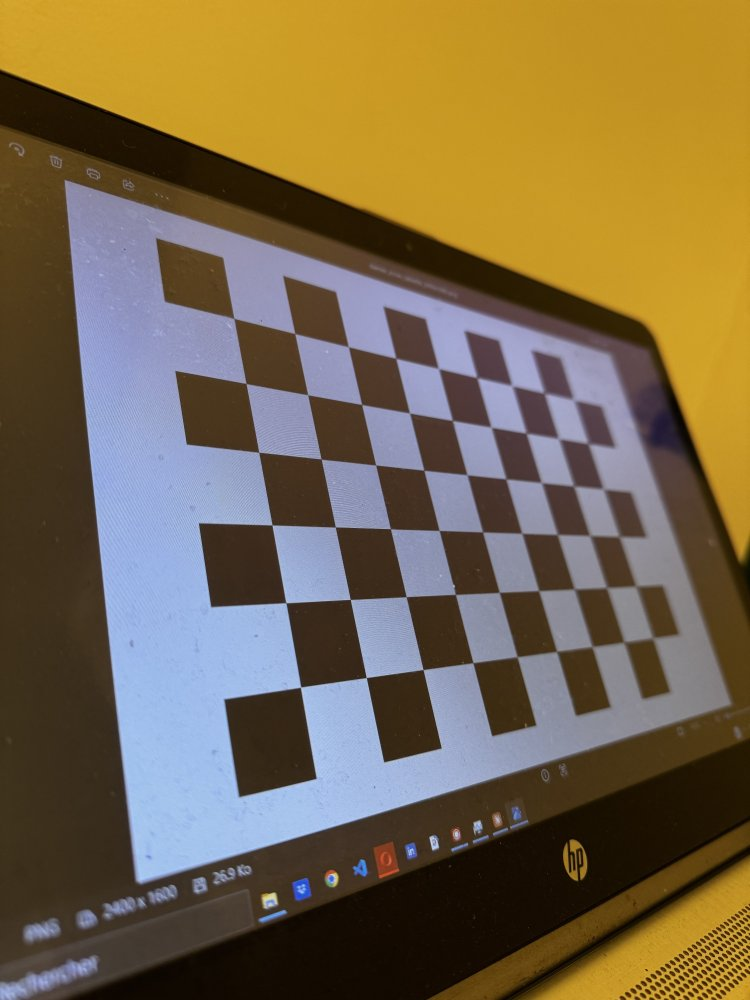
\includegraphics[width=\linewidth]{figures/img3280.jpg}\caption{IMG\_3280, écartée}\end{subfigure}\hfill
\begin{subfigure}{0.24\textwidth}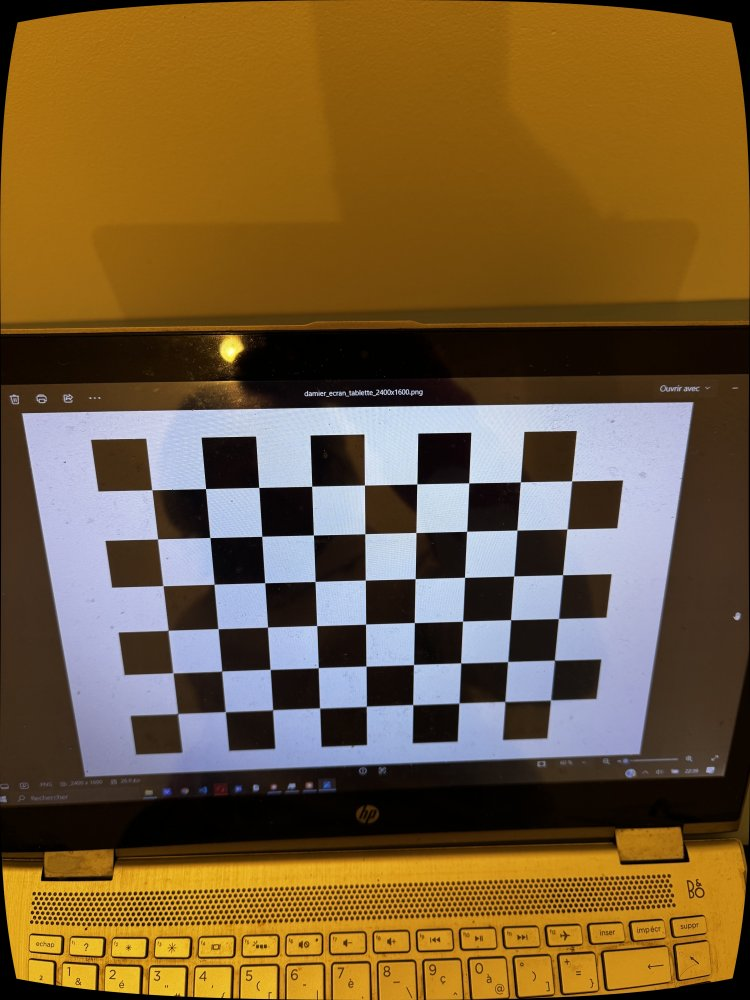
\includegraphics[width=\linewidth]{figures/corrigee.jpg}\caption{Image corrigée}\end{subfigure}\hfill
\begin{subfigure}{0.24\textwidth}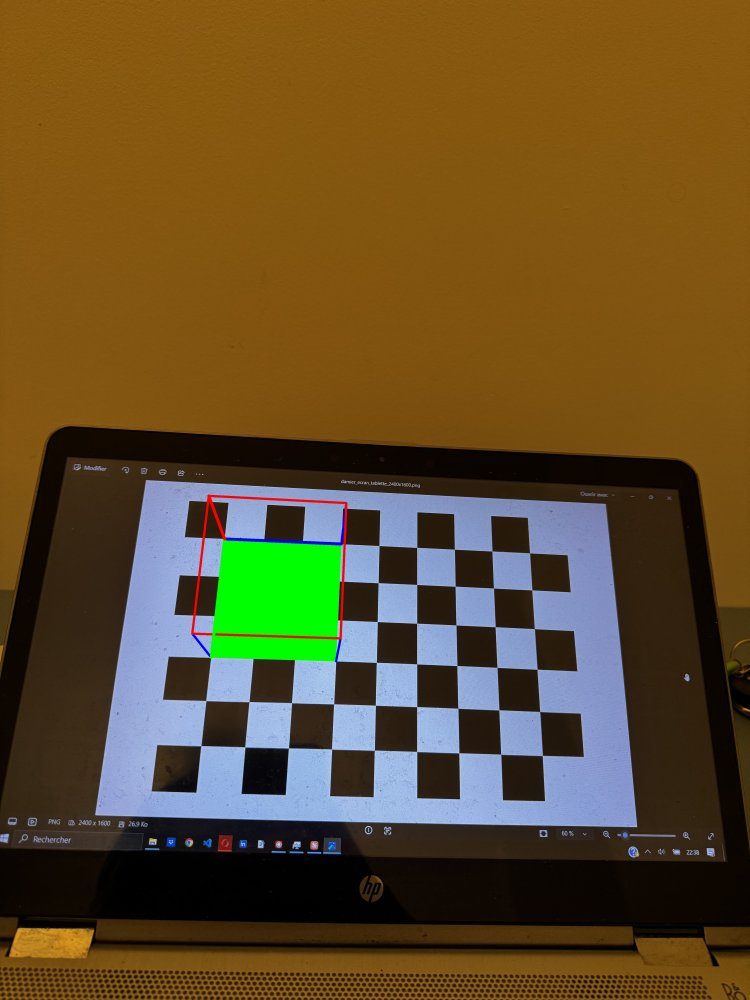
\includegraphics[width=\linewidth]{figures/pose_0.jpg}\caption{Pose, IMG\_3268}\end{subfigure}\hfill
\begin{subfigure}{0.24\textwidth}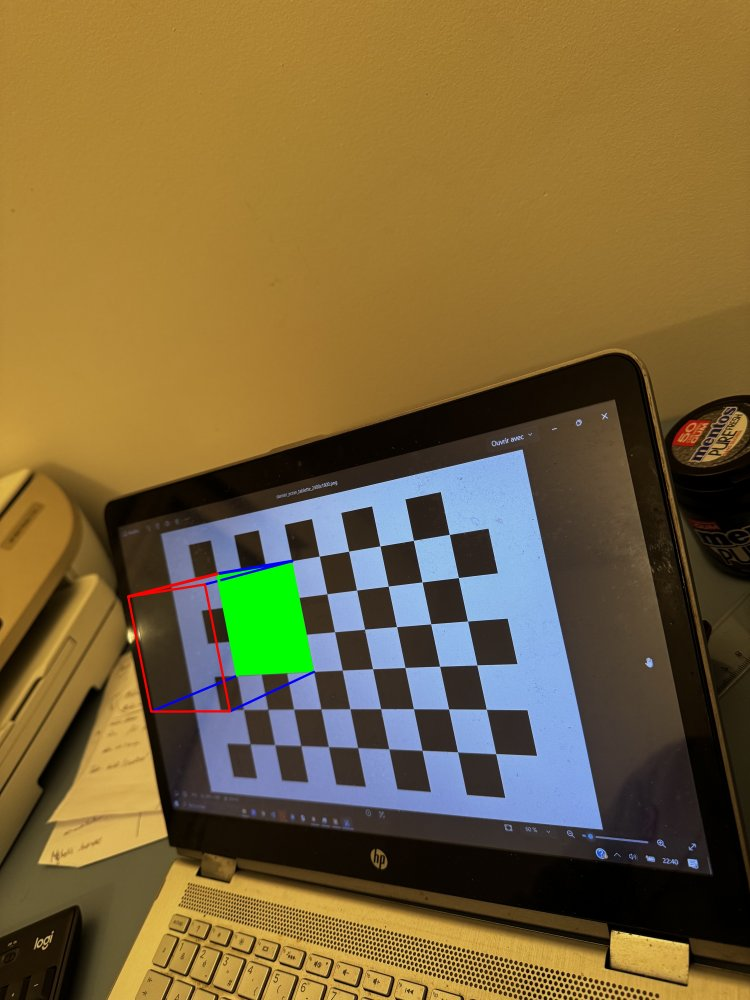
\includegraphics[width=\linewidth]{figures/pose_13.jpg}\caption{Pose, IMG\_3283}\end{subfigure}
\caption{(a) La vue rasante retirée de la calibration. (b) Image IMG\_3269 après correction de la distorsion. (c, d) Cube de 3 cases de côté projeté avec la pose estimée.}
\label{fig:images}
\end{figure}

\section{Discussion}

\paragraph{Écart avec la focale constructeur.} Ma mesure (7,05~mm) dépasse de 4~\% la focale indiquée dans les EXIF (6,765~mm). Je vois trois causes possibles. D'abord, la focale EXIF est la focale nominale, mise au point à l'infini. Or la calibration mesure la distance entre le centre optique et le capteur au moment de la prise de vue, et la mise au point automatique se faisait sur le damier, situé entre 32 et 41~cm. La formule de conjugaison donne alors $d' = f\,d/(d-f) = 6{,}765 \times 361/(361-6{,}765) \approx 6{,}89$~mm, ce qui explique à peu près la moitié de l'écart. Ensuite, la conversion en millimètres repose sur la taille du capteur que j'ai supposée : une erreur de 1~\% sur la taille des photosites donne 1~\% d'erreur sur $f$, alors que $f_x$ en pixels n'en dépend pas. Enfin, l'image que je calibre n'est pas celle du capteur. Le passage de 8064 à 5712 pixels de haut ne correspond pas à un regroupement entier de photosites, donc l'image est rééchantillonnée, et le traitement d'Apple corrige probablement déjà une partie de la distorsion. Je ne peux pas le vérifier sans photo RAW.

\paragraph{Distorsion.} Les coefficients radiaux sont grands et de signes alternés ($k_1>0$, $k_2<0$, $k_3>0$). Pris séparément, ils n'ont pas beaucoup de sens : ils se compensent en partie, et ils sont mal contraints parce que le damier n'occupe jamais les coins de l'image. Pour bien estimer la distorsion en bord de champ, il faudrait des vues où la mire touche les bords.

\paragraph{Taille de la case.} La taille de la case (19~mm, mesurée à la règle) n'intervient pas dans $K$, puisque changer l'échelle de la mire change seulement les translations. En revanche, elle se reporte directement sur les distances : une erreur de 0,5~mm sur la case donne environ 2,6~\% d'erreur, soit à peu près 1~cm à 36~cm.

\paragraph{Pose à partir de points coplanaires.} Les 54 coins du damier sont coplanaires. L'article de Quan et Lan~\cite{quan} montre qu'à partir de quatre points, la pose est déterminée de façon unique hors configurations critiques, et que leurs méthodes linéaires ne dégénèrent pas dans le cas coplanaire. Avec 54 points et un tirage RANSAC (Fischler et Bolles, cité dans le même article), \texttt{solvePnPRansac} dispose de bien plus de points que le minimum, et le cube projeté tombe correctement sur la mire.

\paragraph{Résolution et qualité.} Les 24~Mpx ne donnent pas 24~millions de détails indépendants. À $f/1{,}78$, la tache de diffraction d'Airy a un diamètre d'environ $2{,}44\,\lambda N \approx 2{,}4$~$\mu$m pour $\lambda=550$~nm, alors qu'un pixel de l'image finale correspond à 1,72~$\mu$m sur le capteur. L'optique étale donc déjà un point sur plus d'un pixel, avant même le traitement et la compression. Une erreur de 0,85~px équivaut à environ 1,5~$\mu$m sur le capteur, du même ordre que cette limite.

\section{Limites et améliorations}

Avec plus de temps, je referais l'expérience avec une mire imprimée et collée sur un support rigide pour éviter le moiré, en bloquant la mise au point (verrouillage AE/AF) pour garder une focale constante. Je prendrais aussi plus de vues où la mire couvre les bords et les coins de l'image, et des photos RAW pour échapper au traitement d'Apple. Une validation croisée, qui recalibre en retirant une image à la fois, donnerait une incertitude sur $f$ au lieu d'une seule valeur.

\begin{thebibliography}{9}
\bibitem{zhang} Z.~Zhang, \og A flexible new technique for camera calibration\fg{}, \emph{IEEE Trans. Pattern Analysis and Machine Intelligence}, 22(11), 2000.
\bibitem{quan} L.~Quan et Z.~Lan, \og Linear N-point camera pose determination\fg{}, \emph{IEEE Trans. Pattern Analysis and Machine Intelligence}, 21(7), 1999.
\bibitem{ocv} OpenCV, tutoriels \og Camera Calibration\fg{} et \og Pose Estimation\fg{}, \url{https://docs.opencv.org/4.x/d4/d94/tutorial_camera_calibration.html} et \url{https://docs.opencv.org/3.4/d7/d53/tutorial_py_pose.html}.
\end{thebibliography}

\end{document}
